% *********************************************************************
% © 2021–2026 Jeremy Sylvestre
%
% Permission is granted to copy, distribute and/or modify this document
% under the terms of the GNU Free Documentation License, Version 1.3 or
% any later version published by the Free Software Foundation; with no
% Invariant Sections, no Front-Cover Texts, and no Back-Cover Texts. A
% copy of the license is included in the appendix entitled “GNU Free
% Documentation License” that appears in the output document of this
% PreTeXt source code. All trademarks™ are the registered® marks of
% their respective owners.
%
% *********************************************************************

\newcommand*{\xmin}{-0.5}
\newcommand*{\xmax}{3.5}
\newcommand*{\ymin}{-0.75}  % keep in mind yscale
\newcommand*{\ymax}{6}

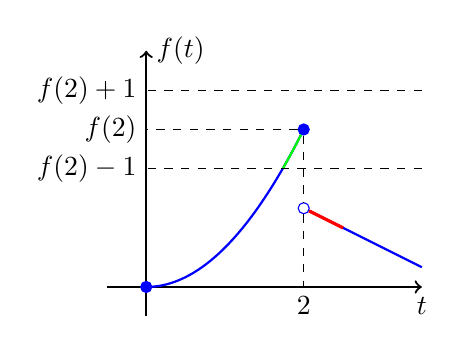
\begin{tikzpicture}
[
	closedpt/.style={circle,draw,fill,inner sep=0pt,minimum size=4pt},
	openpt/.style={circle,draw,inner sep=0pt,minimum size=4pt},
	yscale=0.5
]

	% axes
	\draw[->,thick] (\xmin,0) -- (\xmax,0) node[below] {$t$};
	\draw[->,thick] (0,\ymin) -- (0,\ymax) node[right] {$f(t)$};

	% graph
	\draw[thick, blue, domain=0:2, smooth] plot (\x,{\x * \x});
	\draw[thick, green, domain=1.732:2, smooth] plot (\x,{\x * \x});

	\node[closedpt,blue] at (0,0) {};
	\node[closedpt,blue] at (2,4) (p) {};
	\node[openpt,blue] at (2,2) (l) {};

	\draw[dashed]
		(p) -- (l)
		(l) -- (2,0) node[below] {$2$};
	\draw[thick, blue] (l) -- (3.5,0.5); % slope -1

	\draw[dashed] (p) -- (0,4) node[left] {$f(2)$};
	\draw[dashed] (\xmax,5) -- (0,5) node[left] {$f(2) + 1$};
	\draw[dashed] (\xmax,3) -- (0,3) node[left] {$f(2) - 1$};

	\draw[very thick, red] (l) -- (2.5,1.5);

\end{tikzpicture}
